\chapter{Feder}

Die Feder stellt in der Mechanik ein praktisches Bauteil zur Anwendung
des Hooke'schen Gesetzes. Dieses Gesetzt wurde von Robert Hooke 1678 
fomuliert und beschreibt das elastische Verhalten von Festkörpern,
deren elastische Verformung linear zu angewandten Kraft ist. 
In Verbindung mit dem dritten Newton'schen Axiom (Aktion und Reaktion) 
lässt sich auch eine Federkraft beschreiben welche linear zur Stauchung
ist.

\newpage
\section{Definition}

\begin{figure}[h!]
	\centering
	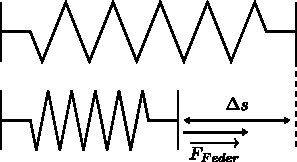
\includegraphics[scale=0.75]{../fig/feder-dehnung.pdf}
	\caption{Veranschaulichung der Federdefinition.}
	\label{fig:feder-dehnung}
\end{figure}

\noindent
Eine Feder kann gedrückt oder gezogen werden, wobei eine Kraft $\vec{F}$ 
entsteht, welche proportional zur Dehnung $\vec{s}$ ist. 
Die Proportionalität wird durch die sogenannte Federkonstante $k$ 
beschrieben. Dies wird auch als Hook'sches Gesetz bezeichnet.

\[ \boxed{\vec{F}_{Feder} = k \cdot \vec{s}} \]

\noindent
Die Richtung der Kraft ist hierbei stets entgegen der Dehnung, d.h. wird die
Feder gestreckt, so zeigt die Kraft zur Feder hin und wird die Feder
gestaucht, so zeigt die Kraft von der Feder weg.

\section{Energie}\label{sec:feder-energie}
Die Energie einer Feder ist definiert als die Federkonstante $k$ multipliziert
mit dem Integral der Dehnung (Weg $\Delta \vec{s}$ bzw. $\vec{s}$).
\begin{figure}[h!]
	\centering
	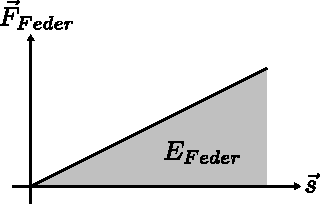
\includegraphics[scale=0.9]{../fig/feder-energie.pdf}
	\caption{Energie einer Feder als Fläche dargestellt.}
	\label{fig:feder-energie}
\end{figure}

\[ \boxed{E_{Feder} 
	= k \cdot \int_{\vec{s}_a}^{\vec{s}_b} \vec{s} \cdot d\vec{s} 
	= \frac{1}{2} \cdot k \cdot \vec{s}^2
} \] \\

\section{Kombination}
Federn können nicht nur einzeln sondern auch in Kombinationen vorkommen. 
Hierbei werden im speziellen zwei Fälle unterschieden:

\begin{itemize}
	\item Parallele Anordnung von Federn
	\item Serielle Anordnung von Federn
\end{itemize}

\begin{figure}[h!]
	\centering
	\begin{subfigure}[c]{0.45\textwidth}
		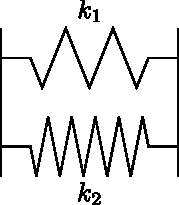
\includegraphics[scale=0.75]{../fig/feder-parallel.pdf}
		\caption{Parallele Federanordnung.}
		\label{fig:feder-parallel}
	\end{subfigure}
	\begin{subfigure}[c]{0.45\textwidth}
		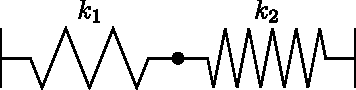
\includegraphics[scale=0.75]{../fig/feder-seriell.pdf}
		\caption{Serielle Federanordnung}
		\label{fig:feder-seriell}
	\end{subfigure}
	\caption{Federanordnungen in Vergleich}
	\label{fig:federanordnungen}
\end{figure}

\subsection{Parallele Anordnung}

\noindent
Werden Federn parallel angeordnet, so können die Federkosntanten summiert 
werden.

\[ \boxed{k_{parallel} 
	= \sum_{i=1}^n k_i 
	= k_1 + k_2 + \dots + k_n
} \]

\subsection{Serielle Anordnung}

\noindent
Werden Federn seriell angeordnet, so können die Federkonstanten reziprok 
summiert werden.
\[ \boxed{\begin{array}{l l}\displaystyle
	\frac{1}{k_{seriell}} 
		&= \displaystyle \sum_{i=1}^n \frac{1}{k_i} = 
		\displaystyle \frac{1}{k_1} + \frac{1}{k_2} 
			+ \dots + \frac{1}{k_n} \\
	& \\
	k_{seriell} 
		&= \displaystyle \frac{1}{\left( 
			\displaystyle \sum_{i=1}^n\frac{1}{k_i}\right)} 
		= \displaystyle \frac{1}{\left(
			\frac{1}{k_1} + \frac{1}{k_2} 
			+ \dots + \frac{1}{k_n} \right)}
\end{array}} \]
Analog zur Elektrotechnik hat ein System bestehend aus zwei Federn
in serieller Anordnung spezielle Verhältnisse zwischen Federkonstanten 
und Energie.
\[ \boxed{\begin{array}{r c l  r c l}
\displaystyle
\frac{E_1}{E_{Total}} 
	&=& \displaystyle \frac{k_1 \cdot {k_2}^2}{k_1 + k_2} 
	\qquad \qquad
	& \qquad \displaystyle \frac{E_2}{E_{Total}}
	&=& \displaystyle \frac{{k_1}^2 \cdot k_2}{k_1 + k_2} \\
 & & & & & \\
\displaystyle \frac{E_1}{E_2} 
	&=& \displaystyle \frac{k_2}{k_1} 
	\qquad \qquad
	& \qquad \displaystyle \frac{E_2}{E_1} 
	&=& 
	\displaystyle \frac{k_1}{k_2}
\end{array}} \]
\section{Federkonstante}
Die Federkonstante ist eine material- und geometrieabhängige Grösse welche
berechnet werden kann mittels des sogenannten Elastizitätsmoduls $E$, der
Querschnittsfläche $A$ und der neutralen Länge $l_0$.

\[ \boxed{k = \frac{E \cdot A}{l_0}} \]

